\section{Local Energy Markets}
\label{sec:lem}

\begin{figure}[htbp]
	\centering
	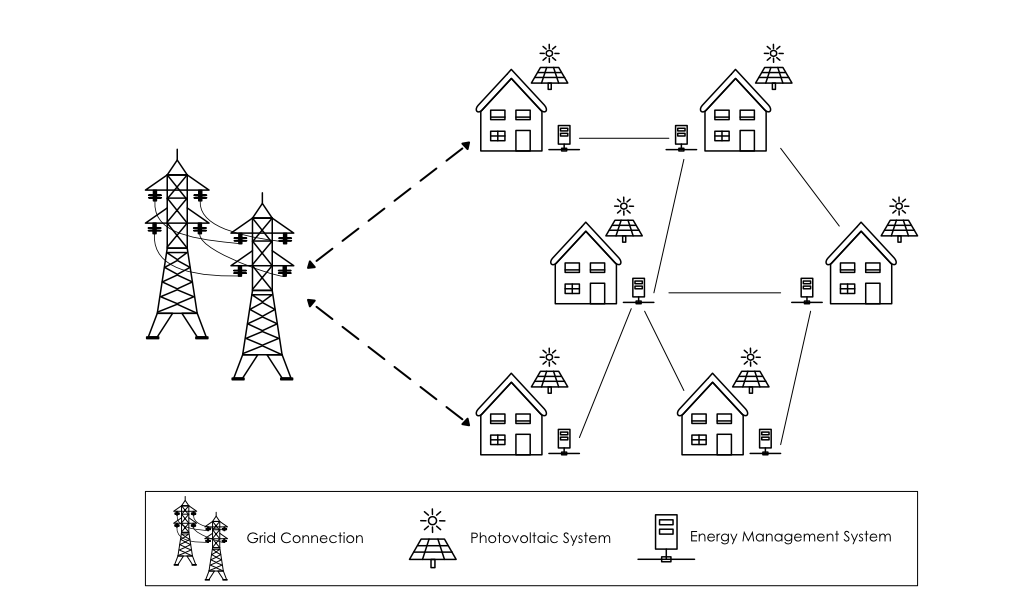
\includegraphics[width=.9\linewidth]{./figures/microgrid_1024x.png}
	\caption{Example of Microgrid setup}
	\label{figure:microgrid}
\end{figure}

To begin with, we revive the stated problem of a successful integration of the increasing amount of
distributed renewable energy sources (RES), as already adressed 
in section \ref{sec:research_motivation}. Due to the centralized generation by large power plants
and the current design of the wholesale markets, the existing grid is not suitable designed
to react in real-time to a significant growing 
amount of distributed RES \shortcite{mengelkamp2018designing} \shortcite{ampatzis2014local}.

In order to successfully integrate and use these RES, new approaches are necessary \shortcite{mengelkamp2018blockchain}.
A possible solution to those technical and market problems is Peer-to-Peer (P2P) energy 
trading in local energy markets (LEM) \shortcite{long2017feasibility}. 

This section will explain the general concept of local energy markets 
and present market components for building efficient LEM. 

In the traditional centralized energy system, large power plants that operate according to a
centralized coordination mechanism, supply a large amount of customer with energy, which are located 
within a wide area (for example a country or a state) \shortcite{mengelkamp2018designing}.

In contrast, decentralized energy systems consists of small-scale energy generators that are 
only used by a small number of people and located close to the energy consumption point \shortcite{mengelkamp2018designing}.
Those local energy markets provide a market platform, market mechanism and market access
for small-scale prosumer and consumer, to trade locally generated energy within their community.
In this case, a community presents a group of geographically and socially close energy agents.
Moreover, all participants buy or sell energy directly with each other by using the provided market platform
without intermediation by conventional energy suppliers \shortcite{zhang2017review}.

In addition, if prosumer have a surplus in electricity, they have the opportunity 
to curtail it, store it in a energy storage device or export it back to the main power grid \shortcite{zhang2017review}.
Considering, in the traditional centralized energy system, trading of energy is mainly unidirectional.
As stated above, the electricity is usually transmitted from large-scale power plants to 
consumers over long distances, while the cash-flow goes the opposite way. 
On the contrary, the P2P energy trading in a LEM encourages multidirectional trading within 
a local geographical community \shortcite{zhang2017review}.

Due to this, LEM promote the consumption of energy close to its generation and, therefore, 
support sustainability and the efficient use of local resources \shortcite{mengelkamp2018designing}.
Furthermore, local energy markets enable (near) real-time pricing and facilitate a local balance
of supply and demand \shortcite{mengelkamp2018blockchain}. 

Further, as stated by \shortciteA{mengelkamp2018designing},
the participants of a LEM do not necessarily have to be physically connected. A virtual microgrid
describes the aggregated control of multiple energy producers, prosumers and consumers in a virtual 
community. Further, the revenue potential can be increased significantly by expanding a physical 
microgrid to inlude virtual participants. 

Referring to \shortciteA{jimeno2011architecture}, a LEM has a specific characteristic
that distinguish it from other aggregation of DER systems. A microgrid has the opportunity
to operate either connected to the main grid or islanded from it. In other words,
this allows a LEM to run disconnected from the main grid, in case it fails or 
the power quality is not satisfactory. Thus, participants of a LEM have a higher quality 
of supply for the loads within it. Additionally, it offers a way of obtaining cheaper 
and cleaner energy for all participants, if elements operated in a LEM taking into 
account by economic and emission policies.

Moreover, P2P energy trading in LEM requires advanced communication and data 
exchanges between the different parties, which makes central management and 
operation more and more challenging. The implementation of LEM needs 
local distributed control and management techniques. \shortcite{andoni2019blockchain}. 
\shortciteA{zhang2017review} stated that, P2P energy trading is often
enabled by ICT-based online services. Moreover, \shortciteA{mengelkamp2018designing} explain that 
the new and innovative blockchain technology as an emerging ICT, 
offers new opportunities for decentralized market designs.
It is designed to enable distributed transactions without 
a central trusted entity.
Accordingly, blockchain can help addressing the challenges faced by 
decentralized energy systems. 

However, blockchain is not a matured technology 
yet and there are several barriers in using them, especially 
for researcher who do not have a technically background. Therefore, this research 
will use a blockchain in the LEM simulation platform as the underlying ICT and will give a
detailed introduction to the blockchain technology in section \ref{sec:about_blockchain}.
In conclusion, the developed simulation platform removes existing technical barriers 
for practicioners and enables the usage of blockchain technology for those.

\subsection{Components of local energy markets}
\label{sec:components_of_local_energy_markets}
\shortciteA{mengelkamp2018designing} developed in his research seven components for a efficient
operation of blockchain-based local energy markets. This subsection will name and briefly 
illustrate each component. Further, the compliance of the developed open blockchain-based
LEM simulation and the seven components will be examined later on in section [ref hinzufügen!!]

\begin{description}
    \item[Microgrid setup (C1):] In general, an explicit objective, a definition of the market 
     participants and the form of the traded energy must be well defined. 
     A LEM can have different, often contradictory objectives. Especially in the
     design of the market mechanism, the implementation of the objective plays an important role.
     Next, a significant number of market participants is needed, who trade energy among each other.
     Moreover, a part of the market participants needs to be able to produce energy. 
     Finally, the form of the traded energy must be described, for example electricity, heat or a 
     combination of them. Additionally, the way of energy transportation must be specified.
     Will be the traditional energy grid used or a physical microgrid build. 
    
    \item[Grid connection (C2:)] The connection points to the superordinate main grid 
     must be well defined. These points measure the energy flows towards the main grid 
     and evaluate the performance of the LEM and can help to balance the energy generation 
     and demand within it. Besides, you have to distinguish between a physical microgrid and 
     a virtual microgrid. A physical microgrid bring along a power distribution grid and is able
     decouple from the main grid, whereas a virtual microgrid simply connects all participants over 
     an information system (C3). Consequently, a virtual microgrid does not have the opportunity
     to physically decouple from the main grid. 
     Nevertheless, to operate in island-mode extensively, a physical microgrid need a large 
     amount of own energy generation capacity and flexibility to ensure supply security and robustness.
         
    \item[Information system (C3):] In addition, all participants must be connected to each other
    and a market platform that monitor all operations must be provided. 
    Therefore, a information system is needed, which should enable equal 
    access for every market participant to avoid discrimination. 
    With reference to \shortciteA{mengelkamp2018designing}, these requirements
    can be implemented by blockchain technology based on smart contracts.
    
    \item[Market mechanism (C4):] Besides, a market mechanism implemented through 
     the information system is necessary. This market mechanism implies the allocation of the
     market and the payment rules. Further, a clear bidding format should be defined. 
     It follows that the main objective of the mechanism is to provide an efficient
     energy allocation by matching the buy and sell orders of the participants appropriately.
     Finally, this should happen in near real time granularity.    
    
    \item[Pricing mechanism (C5):] The market mechanism (C4) includes the pricing mechanism 
     and supports the efficient allocation of energy supply and demand. 
     The traditional energy price is composed in large parts of taxes and surcharges.
     On the contrary, in a LEM different fees come to bear, for example in case of a 
     physical microgrid. Hence, RES typically have almost zero marginal cost, prosumer can 
     price their energy above all appropriate taxes and fees to make profit. 
    Thus, the energy price should linked to the availability of energy. In other words,
    a surplus of energy should lower the LEM energy price while a lack of energy inreases the 
    market price. From an economic point of view, LEM are beneficial to their 
    participants as long as the average energy pirce is lower than the external grid price.
        
    \item[Energy management trading system (C6):] The task and goal of the EMTS
     is to automatically ensure energy supply for a respective market participant.
     Therefore, the EMTS needs access to the energy-related data of the participant, like 
     the real time demand and supply. The EMTS uses this data to forecasts consumption and
     generation and develops a bidding strategy accordingly. 
     Moreover, the EMTS trades the predicted amounts on the provided market platform 
     and aims to maximize the revenue and minimize the energy costs. 
     For this reason, the EMTS needs to have access to the market participant’s
     blockchain account to be capable to automatically perform energy transactions.

    \item[Regulation (C7):] It needs to determined how a LEM 
     fit into the current energy policy and which market design is allowed, how 
     taxes and fees are distributed and billed. Likewise, it needs to 
     determined in which way the local market is integrated into the traditional
     energy market and energy supply system.
     All these emerging issues are specified by the legislative regulation
    
\end{description}

\begin{comment}
    # Mengelkamp \shortcite{mengelkamp2018designing}
    
    An exemplary microgrid energy market scenario of residential consumers and 
    prosumers (consumers with photovoltaic (PV) systems) is shown in Fig. 2. 

\end{comment}

\clearpage